\subsection{平展映射}

定义 2. --- 设 E 与 B 为拓扑空间，\(p\colon\mathrm{E}\to\mathrm{B}\) 为一个映射，\(x\) 为 E 的一个点。我们称映射 \(p\) 在 \(x\) 处是拓扑平展的，如果存在 \(x\) 在 E 中的一个邻域 U 与 \(p(x)\) 在 B 中的一个邻域 V，使得 \(p\) 诱导出从 U 到 V 上的一个同胚。

我们称映射 p 是拓扑平展的，如果它在 E 的每个点 x 处都是拓扑平展的。

当不致产生混淆时 (cf. 下文例 3)，把拓扑平展简称为平展。代替说 \(p\colon \mathrm{E}\to \mathrm{B}\) 是一个平展映射，也可以说 B-空间 \((\mathrm{E},p)\) 是一个平展 B-空间，或者当映射 \(p\) 无疑问时，简单地说 E 是 B 上的一个平展空间。

注. --- 1) 使映射 \(p \colon \mathrm{E} \to \mathrm{B}\) 平展的 E 的点所成的集合是 E 的一个开子集 U，且 p 在 U 上的限制是一个从 U 到 B 的平展映射。

\begin{enumerate}
\def\labelenumi{\arabic{enumi})}
\setcounter{enumi}{1}
\tightlist
\item
  平展映射是连续且开的 (TG, I, p. 33, prop. 5)；特别地，平展映射的像是开的。反之，若 \(p \colon \mathrm{E} \to \mathrm{B}\) 是一个连续且开的映射，且 E 的每个点 x 都有一个邻域 V 使得映射 \(p \mid \mathrm{V}\) 是单射的，则映射 p 是平展的。平展映射的纤维是离散的。
\end{enumerate}

例. --- 1) 设 B 为一个拓扑空间，\((\mathrm{U}_{i})_{i\in\mathrm{I}}\) 为 B 的一族子集。设 E 表示族 \((\mathrm{U}_{i})_{i\in\mathrm{I}}\) 的和空间，\(p: E \to B\) 表示由诸 \(U_{i}\) 到 B 中的典型单射诱导的映射。为使映射 p 是平展的，必须且只需诸 \(U_{i}\) （\(i \in I\) ）都是开的。

\begin{enumerate}
\def\labelenumi{\arabic{enumi})}
\setcounter{enumi}{1}
\item
为使全纯函数 \(f\colon U \to \mathbf{C}\) 是一个平展映射，必须且只需它的导数不取零值。
\item
  代数簇的平展态射 (VAR, R, 5.7.8) 是一个拓扑平展映射，但存在实代数簇的态射，它是拓扑平展的而不是平展态射。例如，映射 \(x \mapsto x^3\) （从 \(\mathbf{R}\) 到 \(\mathbf{R}\) 中）就是这种情形。然而，一个拓扑平展的复解析簇的态射是平展态射 (I, p. 141, exerc. 6)。
\end{enumerate}

命题 6. — 设 X、Y、Z 为拓扑空间，\(f\colon X\to Y\) 、\(g\colon Y\to Z\) 为映射。

\begin{enumerate}
\def\labelenumi{\alph{enumi})}
\item
  设 f 与 g 都是平展的；则 \(g \circ f\) 是平展的。
\item
  设 \(g\) 是平展的，\(f\) 是连续的且 \(g \circ f\) 是开的。则 \(f\) 是开的。
\item
  设 \(g \circ f\) 与 \(g\) 是平展的，且 \(f\) 是连续的。则映射 \(f\) 是平展的。
\item
  设 \(g \circ f\) 是平展的且映射 \(f\) 是连续且开的；则 \(f\) 是平展的，且 \(g\) 在 \(f(\mathrm{X})\) 的每点处是平展的。
\end{enumerate}

我们来证明 (a)。设 \(f\) 与 \(g\) 都是平展的。于是它们都是连续且开的，从而映射 \(g \circ f\) 是连续且开的。设 \(x\) 为 X 的一个点。存在 \(f(x)\) 在 Y 中的一个邻域 W，使得 \(g \mid \mathrm{W}\) 是单射的，并且存在 \(x\) 在 X 中的一个邻域 V，它包含于 \(f(\mathrm{W})\) 中，使得 \(f \mid \mathrm{V}\) 是单射的；于是映射 \((g \circ f) \mid \mathrm{V}\) 是单射的。这就证明了映射 \(g \circ f\) 是平展的 (注 2)。

我们来证明 b)。设 x 为 X 的一个点，W 为 \(f(x)\) 的一个开邻域，使得 g 诱导出从 W 到开集 \(g(\mathrm{W})\) 上的一个同胚。设 V 为 x 的一个邻域，使得 \(f(\mathrm{V})\) 包含于 W 中；于是 \(g \circ f(\mathrm{V})\) 是 \(g \circ f(x)\) 的一个邻域，因此 \(f(\mathrm{V})\) 是 \(f(x)\) 在开集 W 中的一个邻域，从而也是在 Y 中的一个邻域。这就证明了映射 f 是开的 (TG, I, p. 33, prop. 5)。

我们来证明 c)。由 b)，f 是开的。设 x 为 X 的一个点。由于 \(g \circ f\) 是平展的，存在 x 在 X 中的一个邻域 V，使得 \(g \circ f \mid V\) 是单射的。于是 \(f \mid V\) 是单射的，且 f 是平展的 (I, p. 29, 注 2)。

我们来证明 d)。设 \(x\) 为 \(X\) 的一个点，并令 \(y = f(x)\) 。存在一个开邻域 \(V\) （\(x\) 的），使得 \(g \circ f\) 诱导出从 \(V\) 到开集 \(g \circ f(V)\) 上的一个同胚。由于映射 \(f\) 是开的，\(f(V)\) 是 \(y\) 的一个开邻域。映射 \(f|_V\colon V \to f(V)\) （由 \(f\) 过渡到子空间得到）是连续、开且双射的；因此它是一个同胚，从而 \(f\) 在 \(x\) 处是平展的。此外，映射 \(g\) 诱导出从 \(f(V)\) 到 \(g \circ f(V)\) 上的一个同胚，从而在 \(y\) 处是平展的。

推论 1. — 设 B 为一个拓扑空间。从一个平展 B-空间到另一个平展 B-空间的 B-态射是平展的。

这由命题 6 的断言 c) 得出。

推论 2. --- 设 B 为一个拓扑空间；从一个平展 B-空间到另一个平展 B-空间的双射 B-态射是一个 B-同构。

由推论 1，这样的态射是平展的；因此它是开的 (I, p. 29, 注 2)。若它是双射的，则它是一个 B-同构。

推论 3. --- 设 p: E → B 为一个平展映射。p 的每个连续截面都诱导出从 B 到 E 的一个开子集上的一个同胚。

事实上，这样的截面是平展的 (推论 1)，从而是开的。

推论 4. --- 设 p: E → B 为一个平展且分离的映射。设 E 是连通的且 p 有一个截面。则 p 是一个同胚。

设 \(s\) 为 \(p\) 的一个截面；由于 \(p\) 是平展的，\(s\) 的像在 E 中是开的 (推论 3)；它也是闭的，因为 \(p\) 是分离的 (I, p. 27, prop. 3)。由于 E 是连通的，我们有 \(s(\mathrm{B}) = \mathrm{E}\) ，从而 \(p\) 是一个同胚。

命题 7. --- 设 \(p\colon E \to B\) 为一个连续映射。为使映射 \(p\) 是平展的，必须且只需它是开的，且对角线 \(\Delta_{E}\) （\(E \times_{B} E\) 的）在 \(E \times_{B} E\) 中是开的。

首先设映射 p 是平展的。于是它是开的，且 E 的每个点都有一个邻域 V，使得 \(p|V\) 是单射的，这等于说 \((\mathrm{V} \times \mathrm{V}) \cap (\mathrm{E} \times_{\mathrm{B}} \mathrm{E}) \subset \Delta_{\mathrm{E}}\) 。因此 \(\Delta_{E}\) 是 \(E \times_{B} E\) 的一个开子集。

反之，设 p 是一个开映射且 \(\Delta_{\mathrm{E}}\) 是 \(\mathrm{E} \times_{\mathrm{B}} \mathrm{E}\) 的一个开子集。设 x 为 E 的一个点。设 V 为 x 在 E 中的一个开邻域，使得 \((\mathrm{V} \times \mathrm{V}) \cap (\mathrm{E} \times_{\mathrm{B}} \mathrm{E})\) 包含于 \(\Delta_{\mathrm{E}}\) 中。于是 \(p \mid \mathrm{V}\) 是单射的。由 I, p. 29 的注 2，映射 p 是平展的。

命题 8. --- 设

\pandocbounded{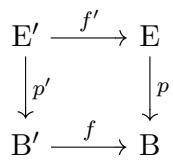
\includegraphics[keepaspectratio]{images/part001_e4ab0ebd.jpg}}

为一个笛卡尔方块。若态射 p 是平展的，则态射 p' 是平展的。反之，若态射 p' 是平展的且态射 f 是普遍严格且满射的，则态射 p 是平展的。

设映射 p 是平展的。特别地，它是开的，且 \(p'\) 是开的 (I, p. 17, prop. 8)。于是考虑笛卡尔方块 (I, p. 13, 例 1)

\[
\begin{array}{c} \mathrm{E} ^ {\prime} \times_ {\mathrm{B} ^ {\prime}} \mathrm{E} ^ {\prime} \xrightarrow {\varphi} \mathrm{E} \times_ {\mathrm{B}} \mathrm{E} \\ \Biggl \downarrow q ^ {\prime} \qquad \qquad \qquad \qquad \Biggl \downarrow q \\ \mathrm{B} ^ {\prime} \xrightarrow {f} \mathrm{B}. \end{array}
\]

我们有 \(\Delta_{\mathrm{E}^{\prime}} = \overline{\varphi}^{1}(\Delta_{\mathrm{E}})\) (loc. cit.)。此外，对角线 \(\Delta_{\mathrm{E}}\) 在 \(\mathrm{E} \times_{\mathrm{B}} \mathrm{E}\) 中是开的 (prop. 7)，从而对角线 \(\Delta_{\mathrm{E}^{\prime}}\) 在 \(\mathrm{E}^{\prime} \times_{\mathrm{B}^{\prime}} \mathrm{E}^{\prime}\) 中是开的。这就证明了映射 \(p^{\prime}\) 是平展的 (loc. cit.)。

现在设映射 \(f\) 是满射且普遍严格的，并设映射 \(p'\) 是平展的。于是 \(p'\) 是开的，因此 \(p\) 是开的 (I, p. 21, prop. 11, \(a\) )。另一方面，\(\Delta_{\mathrm{E}'}\) 是 \(\mathrm{E}' \times_{\mathrm{B}'} \mathrm{E}'\) 的一个开子集。由于 \(\Delta_{\mathrm{E}'} = \overline{\varphi}^{1}(\Delta_{\mathrm{E}})\) 且映射 \(\varphi\) 是满射且严格的 (I, p. 20, def. 6)，\(\Delta_{\mathrm{E}}\) 在 \(\mathrm{E} \times_{\mathrm{B}} \mathrm{E}\) 中是开的。由 prop. 7，映射 p 是平展的。

推论. --- 设 B 为一个拓扑空间。两个平展 B-空间的纤维积是一个平展 B-空间。

设 \((\mathrm{E}, p)\) 与 \((\mathrm{E}^{\prime}, p^{\prime})\) 为平展 B-空间。映射 \(pr_{1}: E \times_{B} E^{\prime} \to E\) 是平展的 (prop. 8)，从而映射 \(p \circ pr_{1}: E \times_{B} E^{\prime} \to B\) 是平展的 (prop. 6, a))。

注 3. --- 设

\pandocbounded{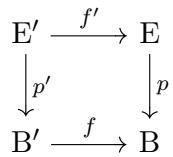
\includegraphics[keepaspectratio]{images/part001_b818a80c.jpg}}

为一个笛卡尔方块。若映射 p 是平展的且映射 f 是严格的，则映射 \(f'\) 是严格的。事实上，在这些假设之下，E 的每个点都有一个开邻域 U，使得 p 诱导出从 U 到开集 \(p(\mathrm{U})\) 上的一个同胚。于是映射 \(p'\) 诱导出从 \((f')^{-1}(\mathrm{U})\) 到 \(f^{-1}(p(\mathrm{U}))\) 上的一个同胚。映射 f 诱导出从 \(f^{-1}(p(\mathrm{U}))\) 到 \(p(\mathrm{U})\) 上的一个严格映射 (I, p. 20)，从而映射 \(f'\) 诱导出从 \((f')^{-1}(\mathrm{U})\) 到 U 中的一个严格映射。由此推出映射 \(f'\) 是严格的 (I, p. 23, 推论 2)。

